\chapter{Background \& Related Work}

According to the International Data Corporation, the size of global data is expected to grow from 33 in 2018 to 175 zetabytes in 2025 as shown in Figure \ref{fig:data_growth}. \cite{IDS} To put that into perspective, the variations in one human genome can be compressed in a lossless fashion to 4 megabytes of data \cite{genome_size}, so the size of our data in 2025 will be equivalent to the digital representation of over 4 quadrillion humans. 

\begin{figure}[h]
\centering
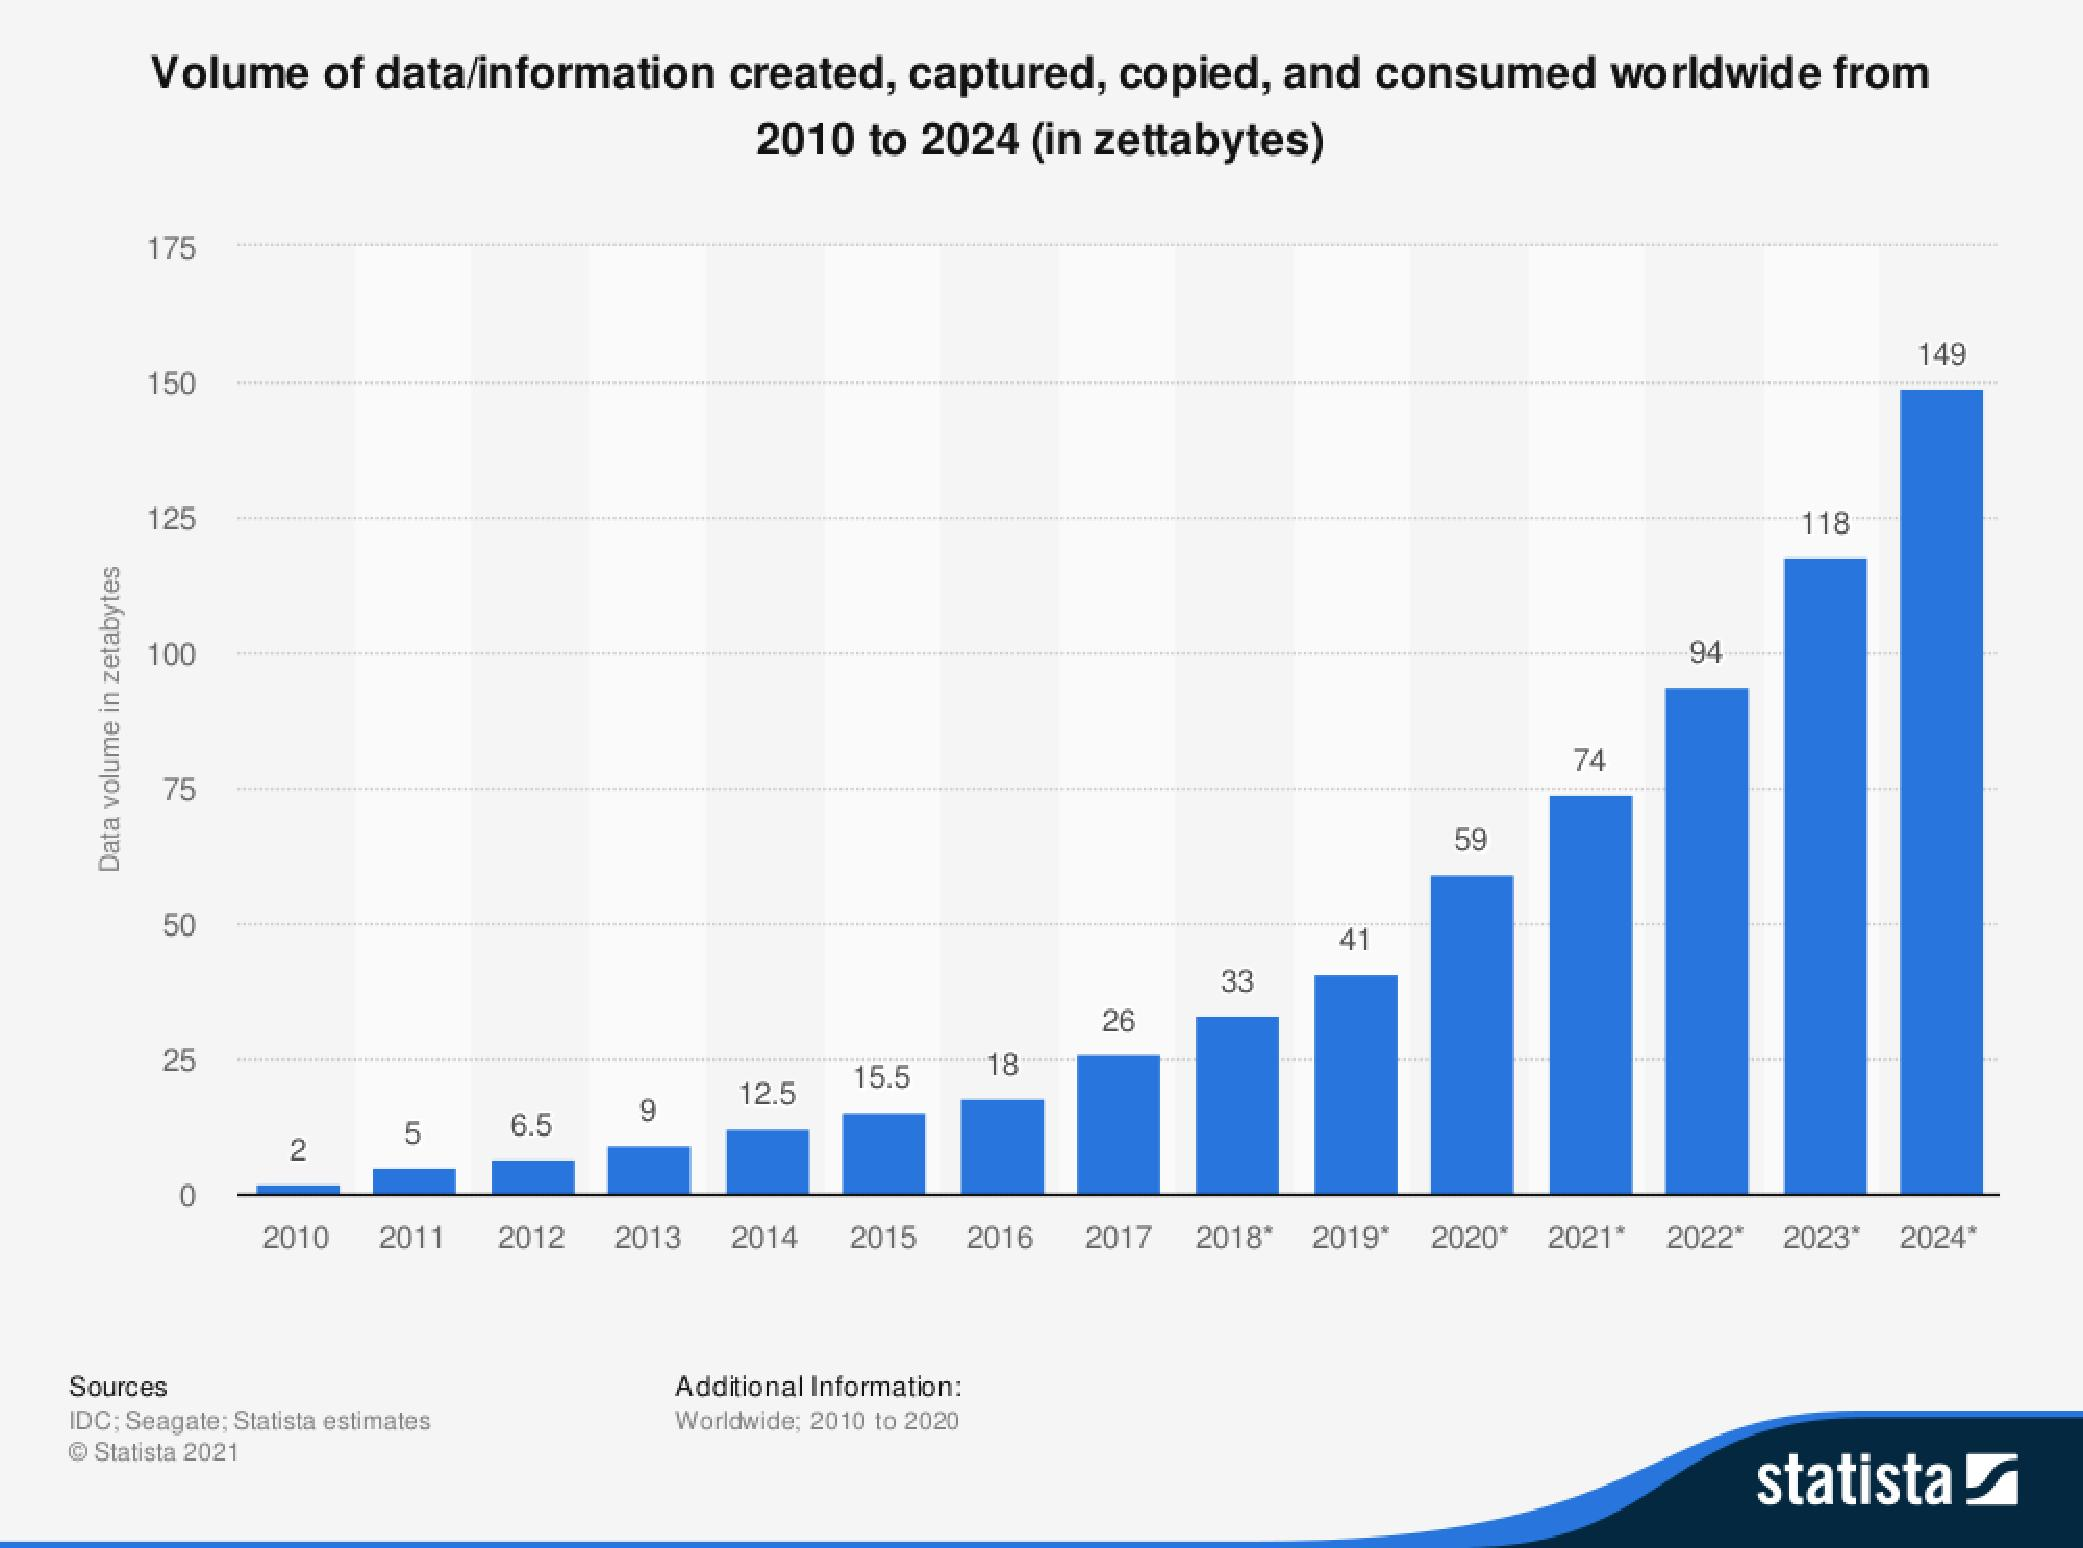
\includegraphics[width=0.5\textwidth]{Figures/global_data_growth.jpg}
\caption{Global Data Growth through 2024. Source: International Data Corporation}
\label{fig:data_growth}
\end{figure}

Along with all of this growth in data comes a growth in the amount of memory with which applications must work. In high performance computing (HPC), we define a computing cluster as a co-located set of computers, each individually called a node, configured for accomplishing a shared task.  Administrators have begun to include "big memory" nodes in these clusters which contain an above average amount of Random Access Memory (RAM) in order to address workloads that require excessive in-memory data. Prominent examples of these workloads include applications that utilize in-memory databases, graph analytics \cite{virtual_memory_tlb}, and large simulations. 

C++ is one of the most popular languages for distributed computing solutions, partly owing owing to the fact that it offers support for useful object-oriented abstractions in conjunction with highly optimized code. \cite{towards_dist_cpp} While much prior work has been dedicated to creating distributed libraries in C++ in \cite{STAPL}  \cite{practical_dist_c}
\cite{taskflow} \cite{intel_tbb} \cite{parallel_programming_w_charm} \cite{chapel} \cite{X10}, other separate work has attempted to improve performance on big memory applications through various optimizations \cite{virtual_memory_tlb}, and still other work has been dedicated to efficiently managing distributed memory \cite{spark} \cite{zookeeper} \cite{memcached} \cite{GAM}  few, if any, attempts have been made to create a library of standard data structures that are designed with big memory capabilities and work loads in mind. Additionally, few general purpose distributed computing libraries are available to the public under open source distribution licenses, as many provide some sort of proprietary value add. This research will be an attempt to create such an open source distributed computing library optimized for big memory utilization, experimenting with novel implementation techniques for standard data structures and drawing from existing literature when necessary. 
\section{Parallel vs. Distributed Computing}
Before detailing the most prominent continuing projects in this space, it is important to draw a distinction between parallel and distributed computing. In order to do that, clear definitions for parallel and distributed computing must be provided. While this thesis project will primarily be geared toward distributed applications running in high-performance computing (HPC) settings, it will also attempt to exploit parallelism, so understanding both is essential for a holistic view of the space in which the proposed project will exist. Definitions included below are a mixture of universal standards used in literature and what will be considered distributed/parallel computing for the purposes of this project.

\paragraph{Parallel Computing}
There are two main modes of parallelism in parallel computing: instruction-level parallelism and thread-level parallelism. Instruction-level parallelism refers to design techniques at the processor/compiler level that speed the execution of sequential programs by allowing individual machine instructions, e.g. additions, floating point multiplications, memory stores/loads, to execute in parallel \cite{ilp_history}. This is typically done using different components of a processor to perform different parts of a given instruction at the same time. Modern processors typically have, at the very least, several floating point units and several integer units, which can handle different parts of the same instruction. The main distinction between instruction-level parallelism and thread-level parallelism is that instruction-level parallelism occurs at the processor level whereas thread-level parallelism exploits concurrency among multiple processors within the same computer \cite{hpc_openstax}.  The thread in thread-level parallelism refers to a thread of execution in which some part of a program runs its code. Threads are different from processes in that threads share the same memory space and are all added to the same existing process. These attributes give threads a distinct advantage over processes when one is working with multiple processors, as an arbitrary number of threads can work on the same shared data structure, either through synchronization or through splitting the structure up into discrete parts \cite{hpc_openstax}. 


\paragraph{Distributed Computing}
The distinction between parallel computing and distributed computing is much like the distinction between instruction-level parallelism and thread-level parallelism. Whereas instruction-level parallelism occurs within one processor while thread-level parallelism occurs in a system with multiple processors, parallel computing occurs within one computer while distributed computing occurs across multiple computers. Naturally, new and unique problems arise when a project migrates from a single system of computers to a cluster consisting of multiple computers that are just as challenging as the problems that arise when making sequential code parallel. Common problems include, but are not limited to heterogeneity in networks, hardware, programming languages, or implementation of standard constructs, openness of components within a distributed system, scalability, fault tolerance, concurrency of different resources across different machines, and unique quality of service (QoS) issues relating to availability, reliability, and performance that do not affect applications running on a single computer \cite{dist_systems_concepts}. Distributed computing can refer to anything from blockchain networks, which distribute verification of information and transactions across many different systems, to web services architectures, in which a web application is broken into modular, discrete components which then run on different computers and communicate across the network, to cloud computing, in which innumerable virtual private servers are spun off and destroyed in tandem across many machines in a massive data center. This project will mainly focus on HPC settings in which memory-intensive scientific applications are run, but hopefully the deliverable will be able to be extended to cloud computing environments, and perhaps even to desktop computer environments if the memory management methods are applicable at this smaller scale. For the purposes of this project, computers with a discrete GPU or other processing component will not be considered distributed computing since many of the aforementioned challenges are less relevant when communicating between components within the same machine - offloading operations to a GPU is analogous to offloading to another CPU core or offloading cache contents to RAM.  
\section{First-Class Distributed Computing in C++}
While the most powerful computers in research in industry continue to expand their processor and GPU counts,
distributed computing is not yet included as a first class component of the C++ STL \cite{towards_dist_cpp}. This forces many developers of high-performance scientific applications to reinvent the wheel for each individual project.  Common parallel computing constructs, like threads, mutexes, and other locks, went through a similar process in C++. Exploring the history of other attempts to standardize distributed data structures, as well as analogous constructs, is essential to understand the full picture of distributed computing in C++. 

\paragraph{Existing Constructs}
Despite the lack of distributed constructs and C++, there are many objects used in heterogeneous/parallel computing that serve as important references for any distributed data structures/algorithms. Most important among the aforementioned constructs are std::async, std::future, and std::thread. \cite{async_cpp}  

\paragraph{Recent attempts}

\section{Memory in Distributed Applications}
Since the beginning of the information era, there has been rapid development of better CPUs with increased cores and faster clock times in conjunction with an increase in demand of data accesses in many applications \cite{sharing_cpu_memory}. Since the affordability and speed of RAM has not followed that of CPUs, this means that the memory resources in a distributed system are now much more expensive relative to CPU cycles. As a result of this, any interventions that improve the efficiency of accessing and sharing memory, whether at an operating system level or user level, could greatly improve the profitability and efficiency of existing distributed applications. Literature presents several existing improvements to memory usage in distributed applications like \cite{virtual_memory_tlb} \cite{sharing_cpu_memory}, this solution is unique in that it attempts to resolve many of the common pitfalls in distributed memory management at a language level. 
\section{Related Work}
\begin{table}[]
\centering
\resizebox{\textwidth}{!}{%
\begin{tabular}{|l|l|l|l|l|l|l|l|}
\hline
Project   & Paradigm & Architecture & Nested & Adaptive & Data Dist. & Scheduling            & Continued development \\ \hline
PC2L      & S/MPMD   & Shared/Dist  & Yes    & Yes      & Auto/User  & ?                     & Yes                   \\ \hline
STAPL     & S/MPMD   & Shared/Dist  & Yes    & Yes      & Auto/User  & Customizable          & Yes                   \\ \hline
PSTL      & SPMD     & Shared/Dist  & No     & No       & Auto       & Tulip RTS             & No                    \\ \hline
Charm++   & MPMD     & Shared/Dist  & No     & No       & User       & prioritized execution & Yes                   \\ \hline
CILK      & S/MPMD   & Shared/Dist  & Yes    & No       & User       & work stealing         & No                    \\ \hline
NESL      & S/MPMD   & Shared/Dist  & Yes    & No       & User       & work and depth model  & No                    \\ \hline
POOMA     & SPMD     & Shared/Dist  & Yes    & No       & User       & pthread scheduling    & No                    \\ \hline
SPLIT-C   & SPMD     & Shared/Dist  & Yes    & No       & User       & user                  & No                    \\ \hline
X10       & S/MPMD   & Shared/Dist  & No     & No       & Auto       & -                     & Yes                   \\ \hline
Chapel    & S/MPMD   & Shared/Dist  & Yes    & No       & Auto       & -                     & Yes                   \\ \hline
Titanium  & S/MPMD   & Shared/Dist  & No     & No       & Auto       & -                     & No                    \\ \hline
Intel TBB & SPMD     & Shared       & Yes    & Yes      & Auto       & work stealing         & Yes                   \\ \hline
\end{tabular}
}
\end{table}
\normalsize
There exist a number of comparable libraries that have attempted to standardize commonly used distributed/parallel structures, or otherwise create a standard library for distributed computing in C++. Out of all of the libraries initially created to address distributed computing in C++, however, few are still in continued development in 2021. The table below compares PC2L, the new proposed solution, to various other attempts to solve the same problem. One additional significant difference not readily visible on the table is that none of these libraries attempt to solve any of the difficulties inherent in memory-bound distributed applications. 



\subsection{STAPL}
\begin{figure}[h]
\centering
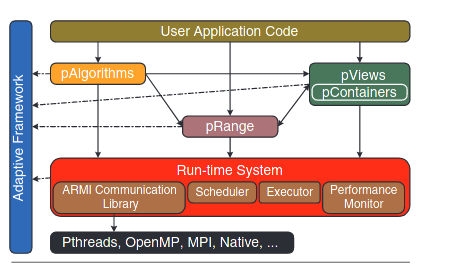
\includegraphics[width=0.5\textwidth]{Figures/stapl_overview.png}
\caption{STAPL Architecture \cite{stapl_parallel_container}}
\label{fig:stapl_arch}
\end{figure}
\paragraph{Description} 
The Standard Template Adaptive Parallel Library (STAPL) was developed by researchers at Texas A\&M University in the late 1990s, far before the C++11 standard provided a set of standardized tools for concurrency. The library was originally created as a super-set of C++'s STL, with the intent to possibly replace the STL on small to medium multiprocessing systems \cite{STAPL}. STAPL is capable of running both single program multiple data (SPMD) and multiple program multiple data applications, and its scheduling algorithm is customizable. STAPL, like the C++ STL, is a generic library, offering data structures and algorithms that can be exploited by a large number of heterogeneous applications. \cite{STAPL}. STAPL implements each distributed data structure as a thread-safe, concurrent object called a pContainer \cite{stapl_parallel_container}. STAPL pContainers consist of a finite collection of typed elements, storage space, and an interface of methods/procedures that can be applied to the pContainer. \cite{stapl_parallel_container} Each pContainer is globally addressable, meaning it provides shared memory address space, and can be composed with other containers to create new structures \cite{stapl_parallel_container}. Distributed data structures implemented by STAPL include an array, a vector, a list, a matrix, a graph, a map, and a set. The library also includes common algorithms for these data structures like those one would find in the C++ STL. STAPL facilitates communication between data structures and algorithms by having algorithms communicate with pViews in the same way that algorithms in the C++ STL communicate with iterators \cite{stapl_parallel_container}. This is done through a pRange object, which is a directed acyclic graph in which vertices represent tasks while edges represent dependencies between tasks.
\textbf{TODO}:  Write some stuff about the runtime system
\cite{stapl_rts}


\paragraph{Contributions} 

STAPL was designed with code translation in mind, so each parallel container within STAPL implements the same methods that would be implemented by its C++ STL counterpart \cite{stapl_parallel_container}. For example, STAPL's implementation of a vector, stapl::pVector, can be accessed, sorted, modified, and constructed using the exact same syntax as a std::vector. STAPL offers users the ability to modify the scheduling algorithm to better suit the needs of their own projects.


\paragraph{Optimizations for memory-bound programs} 

\subsection{Charm++}
\begin{figure}[h]
    \caption{Charm++ Architecture}
    \label{fig:charm_structure}
\end{figure}
\paragraph{Description}
Charm++ is a parallel programming framework designed to ease the development, execution, migration, and decomposition of parallel applications \cite{parallel_programming_w_charm}. Charm++, like STAPL, provides object-oriented abstractions to ease the development of distributed applications. Additionally, in contrast to STAPL, Charm++ provides its own interface for message passing that is inter-operable with MPI. 

\paragraph{Contributions}



\subsection{X10}
    \begin{figure}[h]
        \caption{X10 Architecture}
        \label{fig:x10_arch}
    \end{figure}

\subsection{Chapel}
    \begin{figure}[h]
        \caption{Chapel Architecture}
        \label{fig:chapel_arch}
    \end{figure}

\subsection{Intel Thread Building Blocks (TBB)} 
    \begin{figure}[h]
        \caption{TBB Architecture}
        \label{fig:tbb_arch}
    \end{figure}
